\setcounter{chapter}{-1}% Chapter Template

\chapter{Thesis Organization} % Main chapter title

\label{Chapter0} % Change X to a consecutive number; for referencing this chapter elsewhere, use \ref{ChapterX}

The topic of this thesis is the development of a comprehensively coupled
(supercritical fluid × gas) chromatograph (SFC×GC) and its application to the
analysis of biodiesel. The purpose of this chapter is to clearly and succinctly
explain the content of this thesis and to act as a guide to the reader.

The thesis is divided into five parts, each containing up to three chapters.
Figure~\ref{fig:ThesisOrganization} contains a diagrammatic representation of
its structure.

\begin{description}
 
\item{Part \ref{sec:Part1}}{ provides a scientific background framed in terms of
the molecular basis of sustainability and addresses the question ``Why was the
research done?'' It discusses the climate crisis and constructs an argument 
based on thermodynamics that biodiesel is likely to find a place in its solution
(Chapter~\ref{Chapter1}), explains the use of carbon dioxide as a ''green
chemical'' in analytical chemistry and chromatography and introduces the concept
of SFC×GC (Chapter~\ref{Chapter2}), and describes the chemical properties of a
commercially-viable biodiesel and explains the use of chromatography in the
quality control of biodiesel (Chapter~\ref{Chapter3}).}

\item{Part \ref{sec:Part2}}{ covers the apparatus used and addresses the
question ``How was the research done?'' It describes the development of the
instrumentation used for supercritical fluid chromatography (SFC)
(Chapter~\ref{Chapter4}), explains the need and introduces the theory of fast
temperature-programmed GC and then describes the development of a gas
chromatograph that can perform four temperature\hyp{}programmed
(\SIrange{-20}{350}{\celsius}) runs per minute (Chapter~\ref{Chapter5}).}

\item{Part \ref{sec:Part3}}{ contains the experimental results, and addresses
the question ``What was found?'' It demonstrates the chemical separation of the
main components of biodiesel (Chapter~\ref{Chapter6}), the separation of
biodiesel/petrodiesel blends (Chapter~\ref{Chapter7}), and the promise of using
volatile co-solvents with carbon dioxide in SFC×GC-FID (Chapter~\ref{Chapter8}).}

\item{Part \ref{sec:Part4}}{ contains the concluding Chapter~\ref{Chapter9},
which addresses the question ``What progress was made?'' It reprises the main
argument of the thesis, summarizes the contributions of the research, discusses
its shortcomings, and suggests directions for future research.}

\item{Part \ref{sec:Part5}}{ contains appendices with technical information and the bibliography.} 

\end{description}

\begin{figure}[htbp]
\centering
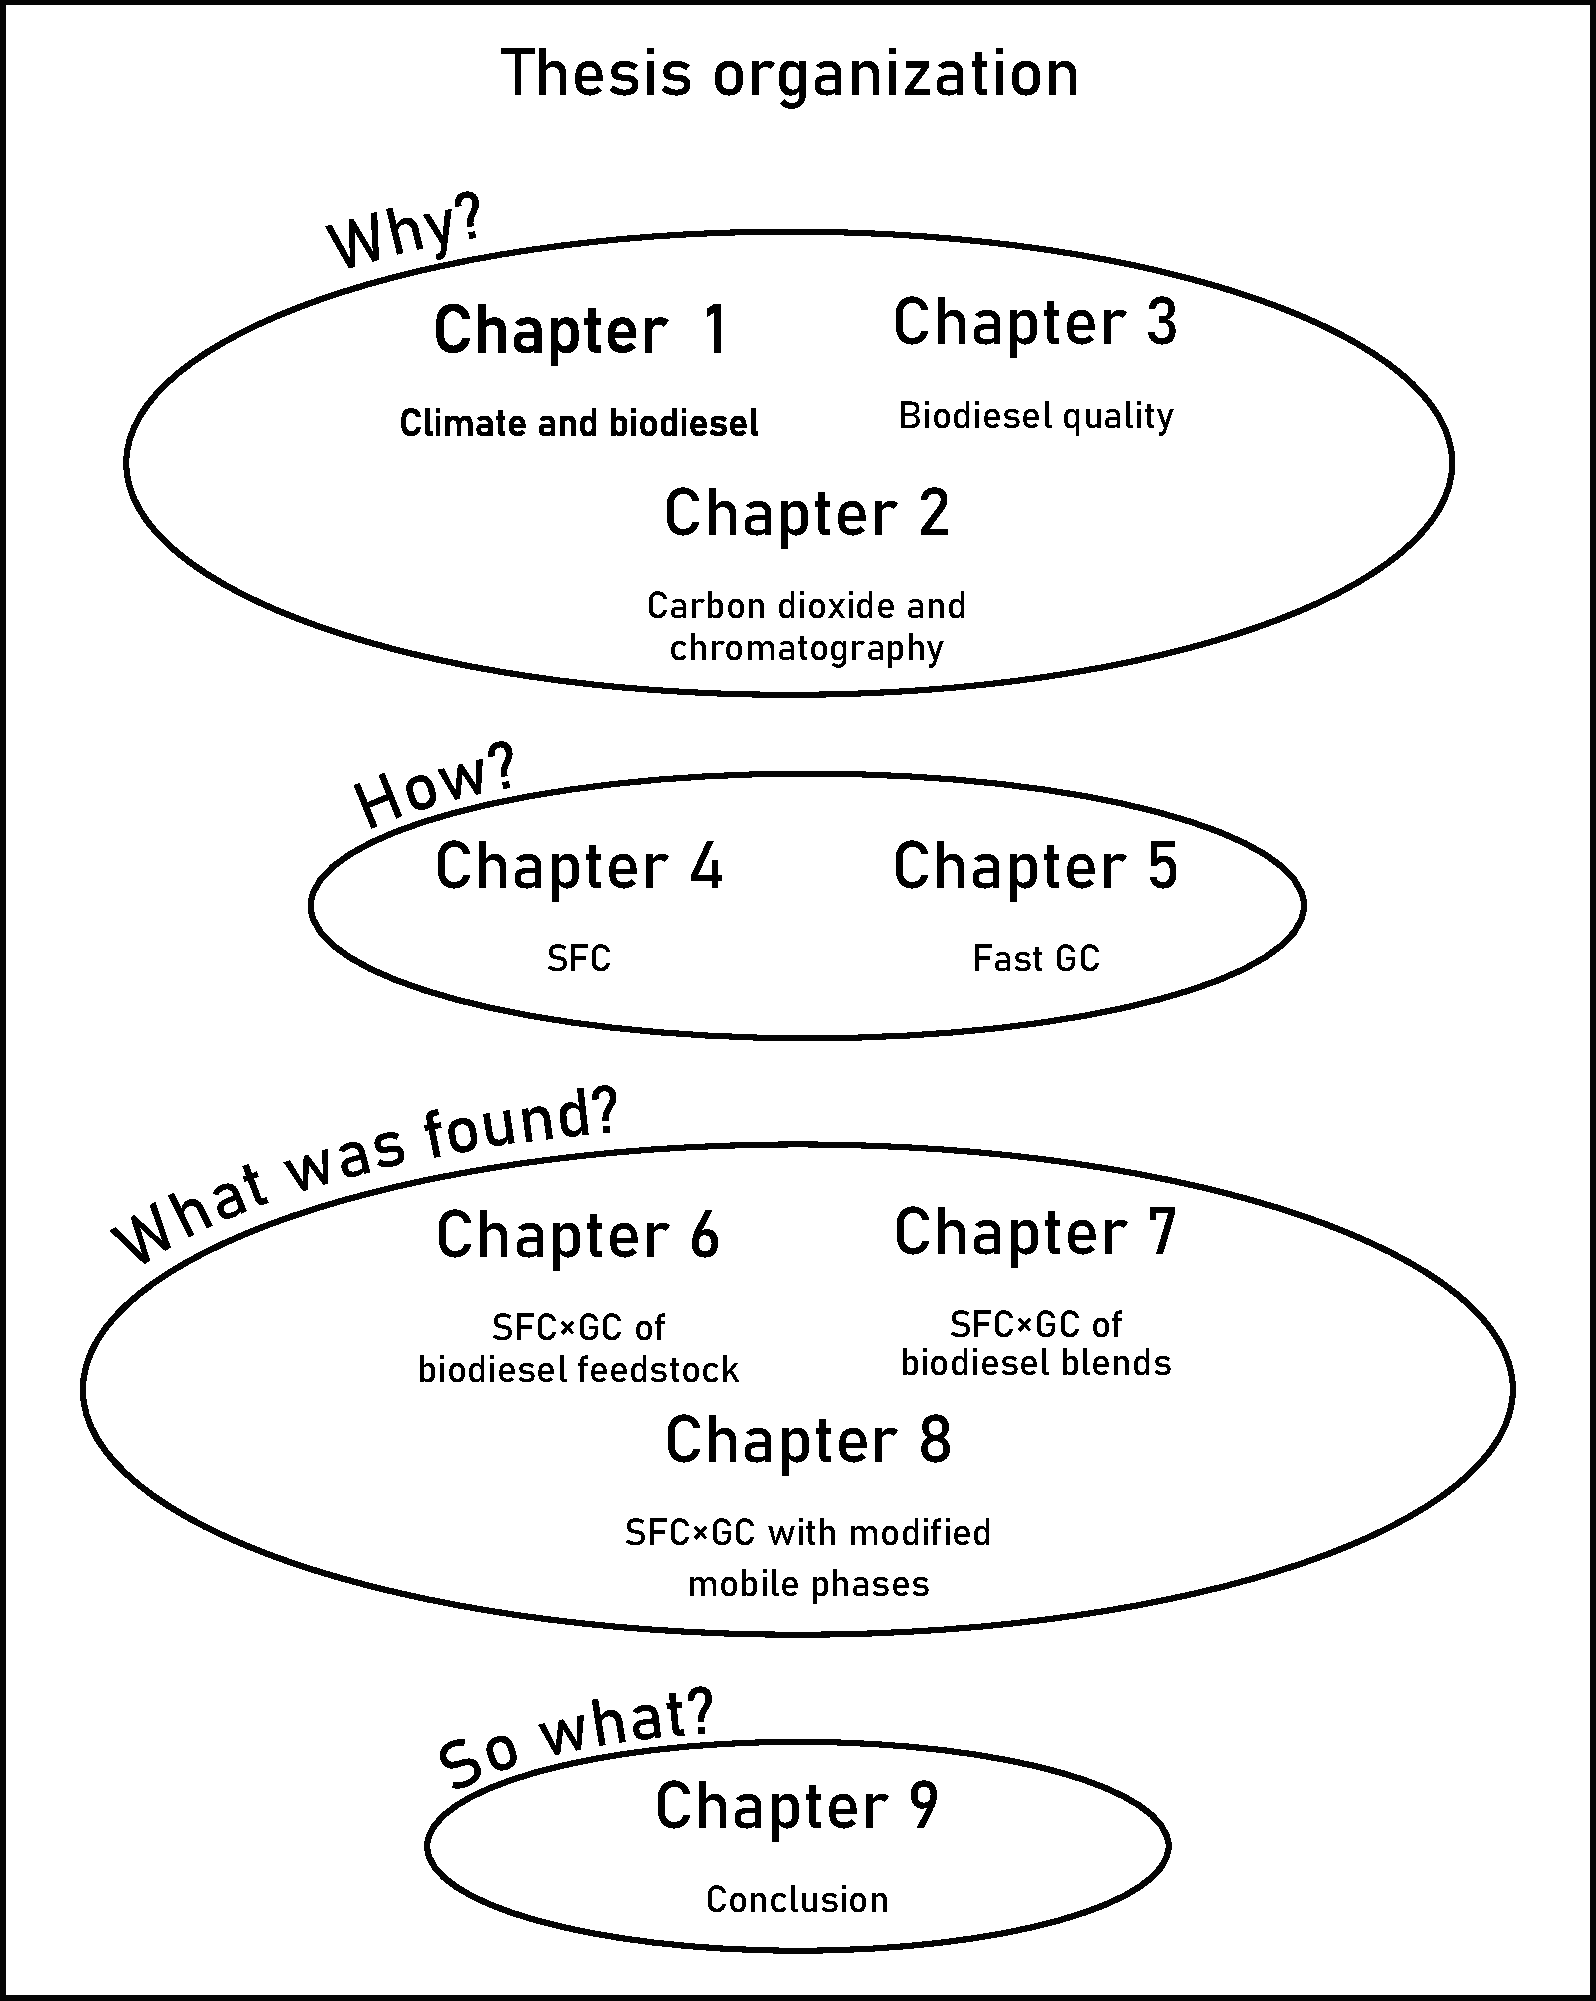
\includegraphics[width=\textwidth]{Figures/ThesisOrganization.pdf}
\decoRule
\caption[Thesis Organization]{A diagrammatic guide to the structure of this thesis.}
\label{fig:ThesisOrganization}
\end{figure}
